\chapter{Galilei relativity}


%~ \Authorline{}
%~ \addtocontents{toc}{\protect\contentsline{section}{{\sl }\smallskip}{}}
%~ \medskip


\thispagestyle{empty}
\newpage

\thispagestyle{empty}
%portrait-of-Galilei
\begin{figure}[H]
\centering
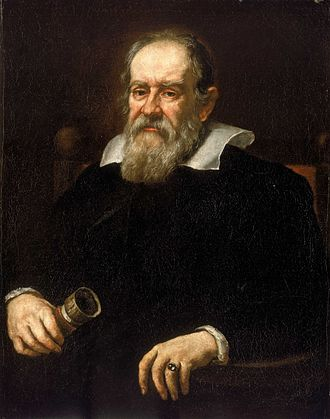
\includegraphics[scale=3]{src/images/lbk-graphics/portraits/galileo-wiki.jpg}
\caption*{Portrait of Galileo Galilei by Giusto Sustermans}
\end{figure}

\begin{small}
\begin{quote}
Galileo Galilei (15 February 1564 - 8 January 1642),
was an Italian astronomer, physicist, engineer,
philosopher, and mathematician who played a major role
in the scientific revolution during the Renaissance.
Galileo has been called the ``father of observational
astronomy'', the ``father of modern physics'', and the 
"father of science". \\\dm \hfill --Wikipaedia
\end{quote}
\end{small}

\newpage %portrait-of-Newton
\thispagestyle{empty}
\begin{figure}[H]
\centering
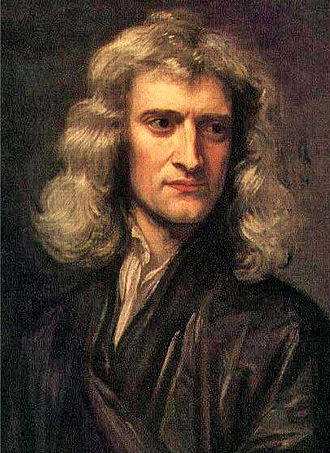
\includegraphics[scale=.5]{src/images/lbk-graphics/portraits/newton-wiki.jpg}
\caption*{Portrait of Newton by Godfrey Kneller}
\end{figure}


\begin{small}
\begin{quote}
Sir Isaac Newton PRS (25 December 1642-20 March\lbk 
1726/27)
was an English physicist and mathematician\lbk 
(described in
his own day as a "natural philosopher") who is widely
recognised as one of the most influential scientists of 
all
time and a key figure in the scientific revolution. 
His book \textsl{Philosophiae Naturalis Principia Mathematica
(Mathematical Principles of Natural Philosophy)}, first
published in 1687, laid the foundations for classical
mechanics. Newton made seminal contributions to optics,
and he shares credit with Gottfried Wilhelm Leibniz for
the development of calculus.
\enlargethispage{1\bsk}
Newton's Principia formulated the laws of motion and
universal gravitation, which dominated scientists' view
of the physical universe for the next three centuries.
\hfill --Wikipaedia
\end{quote}
\end{small}

\newpage

%\renewcommand{\thesection}{1.\arabic{section}}
%~ \renewcommand{\thesubsection}{\thesection 1.\arabic{subsection}}

\section{Absolute space and absolute time}

In his {Principia}, first published in 1686, Newton 
enunciates the basic postulates concerning {the nature 
of 
space and time}. These postulates define what we call 
today 
as the Newtonian spacetime. The part of physics that 
developed for the next two hundred years or so, was 
founded 
on the Newtonian picture of spacetime\footnote{With 
the 
advent of Einstein's special and general theories of 
relativity, today, we have far more satisfactory 
geometrical 
models of spacetime}.

The Newtonian model of spacetime assumes that space and
time are separate and absolute physical entities. They 
are 
considered absolute in the sense that they have 
unchanging
properties. We may quote Newton himself on the 
definition of
space and time\footnote{As quoted in the book 
{Principles of
Relativity Physics}, J. L. Anderson, loc.cit., pp. 
106.}:

{\index{absolute ! space}}
\textit{Absolute space, in its own nature, without 
relation
to anything external, remains always similar and
immovable}.

\index{absolute ! time}\textit{Absolute, true, and
mathematical time, of itself, and from its own nature, 
flows
equably without relation to any thing external.}

\vspace{-.3cm}

\section{Frame of reference}

Recall that a particle is said to be in \textsl{motion} 
if
it changes its position with respect another body 
called a
reference object. In mechanics, we reckon spatial 
position
using an appropriately defined coordinate system 
defined
over the spatial region of interest. A global Cartesian
coordinate system $\{x,y,z\}$ that covers the whole of 
the
Newtonian absolute space is one such reference system. 
 
A reference system is also called a \textsl{reference 
frame}\footnote{See \S~6.4 for further elaboration of 
the notion of a frame of reference.}.

\vspace{-.3cm}

\subsection{The absolute frame}

Newton's absolute space $\mbb{N}$ is a three 
dimensional Euclidean manifold.  In $\mbb{N}$ one may 
introduce a Cartesian coordinate system say, 
$S:\{x,y,z\}$, \index{absolute ! frame} such that 
\textsl{every point} of $\mbb{N}$ is assigned a 
coordinate triplet $(x,y,z)$ in a \textsl{one-to-one, 
continuous} manner.  Further, we assume that the 
coordinate triplet $(x,y,z)$ assigned to a given point 
$P\in \mbb{N}$ in such a coordinate system $S$ is 
\textsl{time-independent}, \ie $P$ would have the same 
coordinates $(x,y,z)$ at all (absolute) times. For this 
reason, one also says that $S$ is \textsl{at rest} in 
$\mbb{N}$.

Such a single (or, global) Cartesian coordinate 
system $S$ at rest in $\mbb{N}$ is called the 
\textbf{Newtonian absolute frame}. 
Later, in chapters 1 and 2, we also introduce 
`\textsl{moving}' Cartesian coordinate systems in 
$\mbb{N}$. Essentially, in a moving coordinate system 
one  assigns \textsl{time-dependent} Cartesian 
coordinates to the points of $\mbb{N}$. We must note 
that, in contradistinction to a moving frame, 
\textbf{the absolute frame is at rest in $\mbb{N}$}. 

\noindent The Euclidean nature of absolute space 
implies
\begin{itemize}
\item The distance between any two points $(x_1, y_1, 
z_1)$ 
and\lbk $(x_2, y_2, z_2)$ is given by
\begin{align}\label{gr.1}
\sqrt{(x_1-x_2)^2+(y_1-y_2)^2+(z_1-z_2)^2}.
\end{align}
\item The angle between any two vectors (directed 
line-segments) $\vec{a}=a_x\eye+a_y\jay+a_z\kay$ and 
$\vec{b} =b_x\eye + b_y\jay + b_z\kay$ is defined (up 
to a 
quadrant) by
\begin{align} \label{gr.2}
\hspace*{-6mm}\cos\theta&=\frac{\vec{a}\dotp\vec{b}}
{\sqrt{(\vec{a}\dotp\vec{a})(\vec{b}\dotp\vec{b})}} =  
 \frac{a_xb_x+a_yb_ y+a_zb_z}
{\sqrt{ (a_x^2+a_y^2+a_z^2)(b_x^2+b_y^2+b_z^2) }}.
\end{align}
\end{itemize}
From the postulated absolute nature of space, it 
follows that the distances and angles (defined above) 
remain unchanged under all physical situations and at 
all (absolute) times.

\vspace{-.3cm}
\section{Newtonian dynamics}

The concept of force is central to Newtonian dynamics. 
One
uses it along with the following \textsl{Newtonian 
postulates}\footnote{In the light of the 
special and general theories of relativity, these 
assumptions are actually wrong and every one of them 
stands 
corrected. One may then wonder if there is a need for 
studying Newtonian mechanics which is based on such 
assumptions. First, we note that these assumptions 
certainly hold in the Newtonian regime ($c\rightarrow 
\infty$) of physics (Cf. \S~1.7) which encompasses a 
major 
part of our physical experience. Even otherwise, one 
may 
profitably study Newtonian dynamics fortified with 
these 
assumptions as a model physical theory of particle 
motion.}, 
on the nature of mass and force 
(particle-interactions), 
to develop Newtonian dynamics. 
\index{Newtonian ! assumptions on force} 
\textsl{Here, we must warn the student that these 
assumptions are strictly Newtonian and are to be used 
with 
caution in situations which are outside the Newtonian 
regime 
of physics\footnote{See \S~1.7 for a discussion of the 
``Newtonian regime of physics.''}}.

\hsl{Absolute nature of mass} A material particle has 
the 
same mass and is representable by the same scalar 
(real 
number) in all Galilei and non-Galilei frames of 
reference\footnote{Galilei and non-Galilei frames are 
discussed in chapters 1 and 2.} . 

\hsl{Absolute nature of force} Force is an absolute 
quantity 
and is representable by the same (three-dimensional 
Euclidean) vector in all Galilei as well as 
non-Galilei 
frames.

\hsl{Action at a distance\index{action at a distance}} 
Interactions between particles are 
\textsl{actions-at-a-distance}. When two particles 
interact, 
the force due to one particle is assumed to act 
\textsl{instantaneously} on the other particle, 
irrespective 
of the spatial separation between them.

\vspace{-.3cm}
\section{Newton laws of motion} 
\index{Newton laws of motion} Newton defined and used 
the absolute frame (see \S 1.2.1) to enunciate his 
laws of motion\footnote{Note that Newton referred to 
the motion of objects relative to the absolute frame 
as {absolute motion}. However, throughout this 
discussion, we use the word absolute to refer to a 
quantity which does not change under a change of frame 
of reference. Therefore, to avoid any possible 
misunderstanding, in this chapter, one may replace the 
Newtonian terms such as 'absolute-motion', 
'absolute-velocity', 'absolute-acceleration' etc., 
with 
'absolute-frame-motion', 'absolute-frame-velocity', 
'absolute-frame-acceleration' etc.}. Newton laws of 
motion quantify  motion relative to the absolute 
frame. 
These laws govern the motion of free 
particles as well as particles moving under the 
influence of forces as referred to the absolute frame. 
In these laws, stated below, the parameter $t$ is the 
absolute time, the vectors
\begin{align*}
\vec{r},\quad \vec{u}\equiv \dv{\vec{r}}{t}\quad \text{
and }\quad \vec{a} \equiv \dv{\vec{u}}{t},
\end{align*}
are, respectively, the position, velocity and 
acceleration
of a point particle $P$ relative to the absolute frame, 
$m
$ and $\vec{F} $ are the mass of $P$ and the force 
acting
on the particle.

\hsl{First law} The absolute frame-velocity of a 
free-particle is a constant in (absolute) time:
\begin{align}\label{gr.3}
\vec{u}\equiv \dv{\vec{r}}{t} = \text{constant 
whenever} 
\; \vec{F}=0.
\end{align}

\hsl{Second law} The application of a force $\vec{F}$ 
to a material particle $P$ produces an 
absolute-frame-acceleration $\vec{a}$ as governed by 
the differential equation
\begin{align}\label{gr.4}
\dv{}{t}(m\vec{u}) =\vec{F}.
\end{align}
Since the mass of the particle is a constant in 
time\footnote{We do not consider the 
\textsl{misleading} case $\sdv {m}{t}\neq 0$ of 
`\textsl{variable mass systems}' here. See 
https://physics.stackexchange.com/questions/53980/
secon 
d-law -of-newton-for-variable-mass-systems.}, we may 
reduce the above equation to
\begin{align}\tag{{1.4b}}
m\vec{a}=\vec{F}.
\end{align}

https://physics.stackexchange.com/questions/53980/
second-law
% -of-newton-for-variable-mass-systems
% 
% Allow me to  quote  from another source:
% 
% "The formulation of Newton's second law as the time 
% derivative of the momentum allows the possibility of 
a 
% variable mass and it was popular in textbooks decades 
ago 
% because it was then in the vogue to consider that, 
according 
% to special relativity, mass depended on velocity 
(e.g., 
% Sears, 1958). Since then, it has been recognized that 
the 
% concept of mass dependence on velocity can be 
misleading, 
% and it is nolonger favored (see Adler, 1987, for an 
% excellent discussion on this subject). 
% 
% Here is an  apparent paradox:
% 
% If we consider the simple case of a variable mass, 
and we 
% write Newton's second law as:
% \vec{F}=m d\vec{v}/dt +\vec{v} dm/dt 			(2)
% we can easily see that it violates the relativity 
principle 
% under Galilean transformations. When \vec{F} is zero, 
in 
% particular, Equation (2) implies that the particle 
will 
% remain at rest in a system where it is originally at 
rest, 
% but it will be accelerated by the "force" -\vec{v}( 
dm/dt)  
% in a system where the particle moves with velocity 
$\vec{v} !$

\hsl{Third law} If two particles $P_1$ and $P_2$ exert
forces on each other, and if $\vec{F}_{21}$ is the 
force
exerted by $P_2$ on $P_1$ and $\vec{F}_{12}$ that due 
to
$P_1$ on $P_2$, then,
\begin{align}\label{gr.5}
\vec{F}_{21} = -\vec{F}_{12}.
\end{align}
Here, we must remember that Newtonian forces are 
actions-at-a-distance and hence are simultaneous (see 
\S 
1.3). One also says $P_1$ {acts on} $P_2$ with the 
force 
$\vec{F}_{12} $ while $P_2$ {reacts on} $P_1$ with the 
force 
$\vec{ F_{21}}$. Then, we may say that the 
\textsl{forces of 
action and reaction are equal and opposite}. Note that 
one 
could also have said that $P_2$ {acts on} $P_1$ while 
$P_1$ 
{reacts on} $P_2$. Thus, in a two-particle interaction, 
if 
one force is called the action, the other is called 
the 
reaction and vice-versa.

\vspace{-.3cm}
\section{Galilei transformation}
\index{transformation ! Galilei}

\hsl{Moving frames of reference}
\index{moving frame}
Let $S:\{x,y,z\}$ be the absolute frame. We define a 
new coordinate system $S^\bst:\{x^\bst, y^\bst, 
z^\bst\}$\lbk through the transformation
\begin{align} \label{gr.6}
x^\bst &= x^\bst (x,y,z,t), \; y^\bst = y^\bst
(x,y,z,t), \; z^\bst =z^\bst (x,y,z,t),
\end{align}
where $x^\bst, y^\bst$, and $z^\bst$ are differentiable 
functions functions of $S$-frame space-coordinates $x, 
y, z$ and the time $t$ \textbf{which, being absolute, 
is the same in $S$ as well as $S^\bst$}. Because the 
new coordinates defined in \eqref{gr.6} depend on the 
absolute time $t$ also, one calls $S^\bst:\{x^\bst, 
y^\bst, z^\bst\}$ a \textsl{moving coordinate system}, 
\index{moving coordinate system} or, a \textsl{moving 
frame of reference}. 
 \index{moving frame}
\hsl{Galilei transformation} Now, we consider a 
specific form for Eqn.\eqref{gr.6} which yields an 
important class of moving frames called \textsl{Galilei 
frames}. Let $S : \nt\{x,y,z\}$ be the absolute frame 
and $S^\bst: \nt \{x^\bst,y^\bst, z^\bst \}$ be a frame 
which moves relative to $S$ as a rigid body in pure 
translatory (i.e., without rotation) motion with the 
{constant velocity} $\vec{v} =v_x\,\eye +v_y\,\jay + 
v_z\,\kay$. Also, we assume that  the origins of the 
two frames $S$ and $S^\bst$ coincide at time $t=0$. 
However, note that we have not assumed that the axes of 
$S^\bst$ are parallel to the corresponding axes of $S$ 
initially.

As  the frame $S^\bst$ is assumed not to rotate 
relative to $S$, the three coordinate axes of $S^\bst$ 
remain parallel to themselves (See \figref{fig1.1}.) at 
all times $t$ as $S^\bst$ moves relative to $S$. 
Further, since the point $O^\bst$ moves with the 
(uniform) velocity $\vec{v}$ relative to $O$, and since 
$O^\bst$ and $O$ coincide at $t=0$, it follows that 
$\vec{OO^\bst}=\vec{v}t$ (\figref{fig1.1}.). If 
$\vec{OP}\equiv\vec{r}$, $\vec{O^\bst 
P}\equiv\svec{r}$, from the (Euclidean) vector-triangle 
$OO^\bst P$ drawn at the instant of time $t$, we note 
that $\vec{O^\bst P} = \vec{OP}-\vec{OO^\bst}$ which is 
the same thing as
\begin{align}\label{gr.7}
\svec{r}=\vec{r} - \vec{v}t.
\end{align}
This is the \textsl{Galilei transformation}.
\index{Galilei ! transformation}
\newpage
\begin{figure}[H]
\begin{center}
\begin{tikzpicture}
% \draw[help lines,step=.25,lightgray] (-4,-4) grid (4,4) ;
% \foreach \y in {-4,-3.5,...,4}
%  \draw (-4.2,\y) node[left]{\tiny\y} ;
% \foreach \x in {-4,-3.5,...,5}
%  \draw (\x,-4.2) node[below]{\tiny\x} ;
\node at (0,0){\ingr{.4}{src/images/lbk-graphics/g-frame.pdf}} ;
 \node at (-1.35,1.25){\small $z$} ;
 \node at (0, .1) {\small $y$} ;
 \node at (-2.,-.6){\small $x$} ;
 \node at (-1.25,-.1) {\small $o$} ;
 \node at (-.05,-.8){\small $\vec{v}t$} ;
 \node at (0.5,1.8) {\small $P$} ;
 \node at (.3,-1.6) {\small $x^\bst$} ;
 \node at (2.2, -2.15) {\small $y^\bst$} ;
 \node at (1.8,-.4) {\small $z^\bst$} ;
 \node at (-.6,1) {\small $\vec{r}$} ;
 \node at (1.25,.4){\small $\svec{r}$} ;
 \node at (1.8,-1.3) {\small $o^\bst$} ;
\end{tikzpicture}
\caption{Schematics of the Galilei transformation}
\label{fig1.1}
\end{center}
\vspace{-.3cm}
\end{figure}

\dfn Any (3-dimensional)  Cartesian coordinate system 
obtained from the absolute frame by a Galilei transformation 
is called a \textsl{Galilei frame}. \index{Galilei ! frame}
\enlargethispage*{1\bsk}

At a given instant of (universal) time $t$, this 
\textsl{passive} transformation, namely, Eqn.\eqref{gr.7}, 
assigns two position vectors $\svec{r}$ and $\vec{r}$ to the 
same point $P$ in absolute space. Here, we may note that a 
passive transformation  $x^i\mapsto x^{\ltip}$  in a space 
$S$ does not move points of $S$ to new points in $S$, but 
only assigns new coordinates to  points of $S$. In contrast, 
an {active} transformation moves points of $S$ to 
corresponding new points in $S$.

The Galilei transformation \eqref{gr.7} is completely 
specified only when it is read together with the general 
assumptions that time, mass and force are absolute 
quantities in Newtonian physics:
\begin{align}\label{gr.8}
t=t^\bst,\quad m = m^\bst,\quad \vec{F} = 
\vec{F}\,^\bst .
\end{align}

Here, the un-starred quantities refer to the absolute frame 
$S$ and the starred ones to $S^\bst$ 
respectively\footnote{The assumptions in Eqn.\eqref{gr.8} 
are made quite generally in Newtonian Physics, even under 
{non-Galilei} transformations between frames of reference. 
See the next chapter.}. Differentiating both sides of the 
Galilei transformation  Eqn.\eqref{gr.7} with respect to 
(the absolute time) $t$, we get
\begin{align}\label{gr.9}
\svec{u} = \vec{u} -\vec{v},
\end{align}
which is the \textsl{Galilei velocity transformation} also 
called \textsl{Galilei velocity addition rule}. 
Differentiating Eqn.\eqref{gr.9} once again with respect to 
$t$, and remembering that $\vec{v}$ is a constant, we get
\begin{align}\label{gr.10}
\svec{a} = \vec{a},
\end{align}
which shows that \textsl{the acceleration of a particle does 
not change under a Galilei transformation}.

\subsection{Galilei invariance of the Newton 
laws}\index{Galilei ! invariance} 

From the third of the assumptions in Eqn.\eqref{gr.8}, it 
follows that $\vec{F} = 0 \Leftrightarrow\svec{F}\hsn = 0$ 
so that if the particle $P$ is force-free in the absolute 
frame, it is force-free in the frame $S^\bst$ also. Also, 
Eqn.\eqref{gr.10} shows that $\vec{a} = 0\Leftrightarrow 
\svec{a} = 0$. Thus, force-free motion is unaccelerated in 
the frame $S^\bst$ also. In other words, the first law of 
motion is valid in every Galilei frame.

Similarly, if we use the postulates $m=m^\bst$ and 
$ \vec{F}\,^\bst$ and the acceleration 'transformation' 
 
\eqref{gr.10} in the equation (1.4b), it follows that  the 
second law of Newton is also true in the frame $S^\bst$. 
Hence we conclude that the second law of Newton holds in 
every Galilei frame.

Finally it also follows from the postulates 
Eqn.\eqref{gr.8} that every algebraic relation between 
forces, and in particular the third law of Newton, remains 
true in the frame $S^\bst$ and hence in all Galilei frames.

Collecting these observations together, we arrive at the 
following:

\thm All the three laws of Newton hold in every 
possible Galilei frame.

\exm A boat which can move with a speed $v_b$ in 
still-water crosses a river of width $w$ in a time $t$ 
along the shortest possible path from one bank to the 
other. Assuming that the river flows steadily with the 
speed $v_r$ relative to the bank-frame, calculate the  
velocity of the boat relative to the bank-frame.

\textsl{Solution}: Let $S$ be the bank-frame  
(\figref{fig1.2} (a)) in which the river flows with the 
steady speed $v_r$, say, along the positive $x$-axis of 
the bank-frame $S$. Then, the velocity of the river 
relative to $S$ is $\vec{v}_r = v_r\,\eye$. 

Let $S'$  (\figref{fig1.2} (b)) be the `rest-frame' or 
the 'still-water' frameof the river in which the river 
appears like a stagnant pool of water. Obviously $S'$ 
has the velocity $\vec{v} \equiv \vec{v}_r$ relative to 
the frame $S$. 

\begin{figure}[H]
\centering
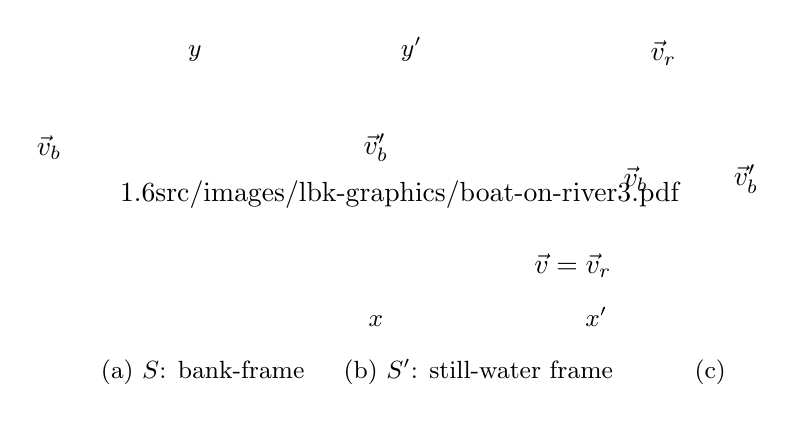
\begin{tikzpicture}
% \draw[help lines,step=.25,brown] (-4.5,-4) grid 
% (4.5,2.5);
% 
% \foreach \y in {-4,-3.5,...,2.5}
%  \draw (-4.75,\y) node[left]{\small \y} ;
% 
% \foreach \x in {-4.5,-3.5,...,4.5}
% \draw (\x,3.1) node{\small \x} ;
\node at (0,0){\ingr{1.6}%
{src/images/lbk-graphics/boat-on-river3.pdf}};
\node at (-2.6,1.8){\small $y$} ;
\node at (.15,1.85){\small $y'$} ;
\node at (-.3,-1.6){\small $x$} ;
\node at (2.5,-1.55){\small $x'$} ;
\node at (-2.5,-2.25){\small (a) $S$: 
\text{bank-frame}} ; 
\node at (4,-2.25){\small (c) $ $} ;
\node at (1,-2.25){\small (b) $S'$: \text{still-water 
frame}} ;
% \node at (-3.5,0) {\small $S$-\text{frame}} ;
\node at (-4.45,.6) {$\vec{v}_b$} ; 
\node at (3,.2) {$\vec{v}_b$} ;
\node at (4.4,.2) {$\vec{v}'_b$} ;
\node at (-.3,.6) {$\vec{v}'_b$} ;
\node at (2.2,-.9) {$\vec{v}\hsn=\hsn\vec{v}_r$} ;
 \node at (3.35,1.8){$\vec{v}_r$} ;
\end{tikzpicture}
\caption{(a) As seen from the bank-frame $S$. (b) As 
seen from the still-water-frame $S'$.}
\label{fig1.2}. 
\end{figure}

The problem states that the boat crosses the river 
along the shortest path in still water in a time $t$; 
obviously, such a path is perpendicular to the 
direction of river-flow in $S$, and has a width $w$. 
Therefore, the velocity of the boat  in the 
still--water frame (rest frame) $S'$ is   $\pvec{v}_b= 
v'_b\,\jay = (w/t)\,\jay$. \  (cf. \figref{fig1.2} 
(b)). Let the velocity of the boat relative to the 
bank-frame $S$ be $\vec{v}_b$\lbk  (cf. \figref{fig1.2} 
(a)). Then, a Galilei transformation to $S'$ which 
moves with the velocity $\vec{v}\equiv\vec{v}_r$ 
relative to the frame $S$, gives $\vec{v}_b +\vec{v}_r= 
\pvec{v}_b$ (cf. \figref{fig1.2} (c)), Thus, $ 
\vec{v}_b = $ $\pvec{v}_b-\vec{v}_r =$ $ (w/t)\jay 
-v_r\eye$.  This gives $v_b=\sqrt{(w/t)^2+(v_r)^2}$ and 
 $\vec{v}_b =v_b\, \eye $ is the required velocity of 
the boat relative to the bank-frame $S$.%

Example 1.2.  A river flows from west to east with a 
speed  $v_r$. A swimmer who can swim  steadily at a 
speed of $v_0$ in still-water, swims from the south 
bank to the north taking the shortest possible time. 
What should be his swim-direction?

\newpage

\begin{figure}[H]
\begin{center}
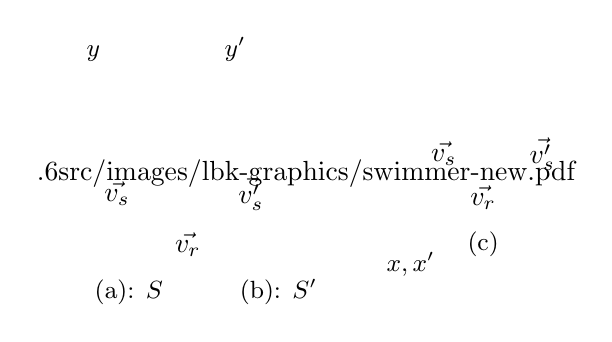
\begin{tikzpicture}
% \draw[help lines,step=.25,brown] (-3,-3) grid 
% (3,2.5);
% 
% \foreach \y in {-3,-2.5,...,2.5}
%  \draw (-4.75,\y) node[left]{\small \y} ;
% 
% \foreach \x in {-4.5,-3.5,...,4.5}
% \draw (\x,3.1) node{\small \x} ;

\node at (0,0)%
{\ingr{.6}{src/images/lbk-graphics/swimmer-new.pdf}};
\node at (-2.7,1.3)[above] {\small $y$} ;
\node at (-.9,1.3)[above] {\small $y'$} ;
\node at (.9,-1.15)[right]{\small $x,x'$} ;
\node at (-2.25,-1.5){\small (a): $S$} ;
\node at (-.35,-1.5) {\small (b): $S'$} ; 
\node at (2.25,-.9) {\small (c)} ; 
\node at (2.25,-.3){$\vec{v_r}$} ;
\node at (1.75,.25){$\vec{v_s}$} ;
\node at (3,.25){$\vec{v'_s}$} ;
\node at (-2.4,-.25) {$\vec{v_s}$} ;
\node at (-.7,-.25) {$\vec{v'_s}$} ;
\node at (-1.5,-.9){$\vec{v_r}$} ;
\node at (-2.4 ,-1) {$\gkq$} ;
\end{tikzpicture}
\caption{} 
\label{fig1.3}
\end{center}
\end{figure}

\soln Let $S$ be the bank-frame and let us choose $S$ 
such that the river moves with the velocity $\vec{v} = 
v_r\,\eye$ relative to $S$ (See \figref{fig1.3}). 
 
A swim-event of shortest possible time, here,  is 
evidently a straight-line path perpendicular to the 
river executed with the maximum still-water-speed $v_0$ 
of the swimmer. Therefore, relative to $S'$, the 
velocity of the swimmer along this minimal-time-path is 
given by $\pvec{v}_s\equiv v_0\,\jay$. 

\enlargethispage*{1\bsk}
Now, a Galilei transformation from $S'$ to the 
bank-frame $S$ gives the velocity of the swimmer in the 
bank-frame $S$ to be $\vec{v}_s=\vec{v}_r+\pvec{v}_s$ 
$=v_r\,\eye+v_0\,\jay$. The angle $\theta$ made by 
$\vec{v}$, i.e., the path of the swimmer in the 
bank-frame $S$, with the flow-direction $\eye$ is given 
by $\tan\theta = v_0/v_r$. 
\ebx
\exm{Show that the set of all Galilei boosts form a 
real, 3-parameter, continuous, $ 4\times 4 $ matrix 
group.}\footnote{L. Fonda and G.C. Ghirardi, 
\textsl{Symmetry Principles in Quantum Physics}, Marcel 
Dekker Inc., New York, 1970.} \index{Galilei ! boosts} 
\index{Galilei ! group of Galilei boosts}
 
\soln Observe that with each choice of the constant 
velocity vector in Eqn.\eqref{gr.7}, say, $\vec{v} = 
\vec{v_1}, \; \vec{ v_2}, \dots$, we get a Galilei 
transformation leading to a corresponding Galilei frame 
$S_1$, $S_2$, $\dots$, in each of which Newton laws are 
equally valid.  We denote the set of all Galilei 
transformations by $ {\mathcal{G}(v)} $, and an 
arbitrary Galilei transformation belonging to $ 
{\mathcal{G}(v)} $ by $ G(\vec{v}) $.  We may write, 
symbolically,
\begin{align}\label{9}
G(v): \text{Newton Equations} \mapsto \text{Newton
Equations}.
\end{align}
In other words, a Galilei transformation is a 
continuous function of the vector variable $\vec{v} 
=(v_1,v_2,v_3) $ in the domain $ -\infty< 
v_1,v_2,v_3<\infty $. Clearly, $G(\vec{v})$ is a 
\textsl{symmetry transformation} of the Newton 
equations. The set of all $G(\vec{v})$ form a group 
called the \textsl{the restricted Galilei group} which 
is a three parameter continuous symmetry group of the 
Newton laws of motion. In fact, in addition to the 
three parameter transformations $ G(\vec{v}) $ defined 
in Eqn.\eqref{gr.7}, which we may also call the 
{Galilei boosts}, the general Galilei group includes 
space and time translations and the proper rotations 
which we do not discuss here. We refer the interested 
reader to the book by Fonda and Ghirardi, loc.cit.

\exm Show that the set of all Galilei boosts form a real 
3-parameter continuous matrix group.
\prf An arbitrary Galilei boost 
\begin{align*}
 t^\bst=t,\; x^\bst=x-v_1t, \; y^\bst=y-v_2 t, \; 
z^\bst=z-v_2 t,
\end{align*}
may be written in matrix notation as 
\begin{align}\label{gr.12}
X\mapsto X^\bst ={G}(\vec{v})X,
\end{align}
\begin{small}
where
\begin{align}\label{gr.13}
 X&=\begin{pmatrix} t \\x\\y\\z
\end{pmatrix},
\:X^\bst =\begin{pmatrix} t^\bst
\\x^\bst \\y^\bst \\z^\bst \end{pmatrix} ,\:
{ G(\vec{v})}
=\begin{pmatrix} 1\ph{_2}&0&0&0\\
-v_1&1&0&0\\
-v_2&0&1&0\\
-v_3&0&0&1\\
\end{pmatrix}.
\end{align}
We note the following properties of the Galilei boosts:
\begin{align}
{G(\vec{u})}{G(\vec{v})}=&\begin{pmatrix}
1\ph{_2}&0&0&0\\
-u_1&1&0&0\\
-u_2&0&1&0\\
-u_3&0&0&1\\
\end{pmatrix}
\begin{pmatrix}
1\ph{_2}&0&0&0\\
-v_1&1&0&0\\
-v_2&0&1&0\\
-v_3&0&0&1\\
\end{pmatrix}\notag\\
% \end{align*}
% \begin{align}
=&\begin{pmatrix}\label{gr.14}
1\ph{_2} &0&0&0\\
-(u_1+v_1)&1&0&0\\
-(u_1+v_1)&0&1&0\\
-(u_1+v_1)&0&0&1\\
\end{pmatrix}
={ G(\vec{u}+\vec{v})},\\
{G}^{-1}(\vec{v})=&
\begin{pmatrix} 1&0&0&0\\
v_1&1&0&0\\
v_2&0&1&0\\
v_3&0&0&1\\
\end{pmatrix}={G}(-\vec{v}), \quad \\
{G}(\vec{0})=&
\begin{pmatrix} 1&0&0&0\\
0&1&0&0\\
0&0&1&0\\
0&0&0&1\\
\end{pmatrix}={E}.
\end{align}
Thus the set of all Galilei boosts is a real 3-parameter
continuous $4\times 4$ matrix group (under matrix
multiplication as the group composition) and ${G}
(\vec{0})= {E}$ as the identity.\ebx
 \end{small}
 
 \vspace{-.2cm}
 
 \subsection{Galilei relativity and absolute
velocity}\index{Galilei ! principle of relativity}
The Newtonian statements of the laws of motion 
(Eqn.\eqref{gr.3} to Eqn.\eqref{gr.5}), clearly, hold only 
relative to the absolute frame. However, the 
\textsl{Galilei principle of relativity} brings out an 
important new feature of the Newton laws of motion, namely, 
the validity of Newton laws of motion in all Galilei frames.

The Newtonian absolute frame is the unique 
frame in which the three laws of motion hold. But, the 
Galilei principle of relativity implies that the three laws 
of motion hold not only in the absolute frame, but also 
in every Galilei frame. Thus, it is impossible to 
identify the absolute frame using the Newton laws. More 
specifically, as Newton defines absolute motion as motion of 
objects relative to the absolute space, the failure of 
Newton laws of motion to identify the absolute frame implies 
that Newton laws of motion do not identify the absolute 
space\footnote{Recall that the absolute frame is any 
Cartesian coordinate system \textbf{at  rest} relative to 
the absolute space.}. In particular, it follows from this 
observation that the Newton laws of motion fail to determine 
the absolute velocity of a particle\footnote{The velocity of 
a particle relative to the absolute frame as its absolute 
velocity.}.

\begin{quote}
\textsl{Hence, if physics were to be just the Newton 
laws of motion (and all the other laws that are compatible 
with it), then the Galilei principle of relativity abolishes 
the notion of absolute velocity from physics.}
\end{quote}

\vspace{-.3cm}

\section{Inertial frame in Newtonian\\ mechanics} 
The notion of a \textsl{Galilei frame} (Cf. Definition~1.1 
in \S~1.5) is a  key idea in Newtonian mechanics. Since  all 
the three Newton laws of motion are true relative to the 
Newtonian absolute frame, formally one may regard it also as 
a Galilei frame in the light of the Therorem~1.1 of  \S~1.5. 
Further, in particular, since the first law of Newton, 
also called the law of inertia, holds in every Galilei 
frame one may conclude that:
\begin{quote}
\textsl{A Galilei frame is also called an inertial  frame 
in Newtonian mechanics. It may be worth repeating here 
that, by definition, a \textsl{free particle} moves with 
zero acceleration in a Galilei frame.} 
\end{quote}

The existence of a long range force such as the the 
Newtonian gravitational attraction implies that a given 
particle, at a spatial point, say $P$, in a Galilei frame 
can never be regarded (in principle) as free from the 
Newtonian gravitational attraction due to the rest of the 
matter in the universe. However, Newtonian gravity 
diminishes as we move away from the gravitating matter 
and becomes practically zero if the point $P$ is 
sufficiently far removed from the rest of the matter in 
the universe. Thus, we may say a particle at the point 
$P$ is practically ``isolated'' and is force-free if it 
is \textsl{sufficiently} far removed from the rest of 
the matter in the universe. Thus, frames called local 
Galilei frames (i.e., local inertial frames) may be 
defined in a sufficiently small spatial region around 
a point $P$ in which a test-particle is (practically) 
force-free and (and hence is practically) 
un-accelerated.

\vspace{.2cm}
\dfn A \textsl{local Galilei frame} at a spatial point 
$P$ is a Cartesian coordinate system $S_P$ defined in 
a sufficiently small spatial region $\mbb{R}$ around 
$P$. By choosing the spatial region covered by  $S_P$ 
around $S_P$ to be sufficiently small,  $S_P$ can be 
'made' Galilei to any  given  degree of accuracy (of 
the measurement of acceleration)\footnote{ The `size', 
or the spatial region of validity $\mbb{R}$, of such 
an (approximately) Galilei frame $S_P$, is evidently 
determined by the degree of accuracy of the instruments 
used for the measurement of acceleration. Outside the 
spatial region $\mbb{R}$, the Cartesian coordinate 
system $S_P$ although defined, would not provide a 
Galilei frame in view of a detectable acceleration for 
a free-particle.}.

\vspace{.2cm}
Empirically, it was thought of that a coordinate system 
relative to which the fixed stars are at rest is a Galilei 
frame. Today, we know that our galaxy rotates and the 
universe expands. When such motion of the distant stars is 
taken into account, the frame of the fixed stars may not be 
acceptable as sufficiently Galilei. One may then consider a 
global Cartesian coordinate system in which all other 
galaxies appear (to us) to recede radially from us, as a 
better Galilei frame than the frame of the fixed 
stars\footnote{See R.W.Rindler, loc.cit.}.

\vspace{-.2cm}

\section*{Exercises}

\exise A swimmer has a steady speed of $v_0$ in still water 
swims in a river that flows with the constant speed 
$(v_r,0,0)$ relative to its  bank-frame $S:\nt\{x,y,z\}$. 
Determine the velocity $\vec{v}$ of the swimmer relative to 
 $S:\nt\{x,y,z\}$ as a function of the angle theta made by 
$\vec{v}$ with the $x$-axis.

\exise The equation to the orbit of a particle falling under 
(uniform) gravity along the line $x =0$ of a Galilei frame 
$S:\nt\{x,y,z\}$  is given by $x=0,\; y=y_0+u_yt-gt^2/2$ 
where $y(0)$ $u_y$ and $g$ are constants. Obtain the 
equation to the orbit in the Galilei frame $S'$ related to 
$S$ by the $x$-Galilei-boost $x'=x-vt,\;y=y,\;z'=z$.

\vspace{.2cm}
{\bf{\textit{Reference:}}}

James L Anderson, \textsl{Principles of Relativity
Physics}, Academic Press, New York, 1967, Chapter 5.
